\documentclass[12pt]{article}

\usepackage{amsmath,amsthm,amsfonts,amssymb,amsxtra}
\usepackage{pgf,tikz}
\usetikzlibrary{arrows, calc}
\renewcommand{\theenumi}{(\alph{enumi})} 
\renewcommand{\labelenumi}{\theenumi}

\pagestyle{empty}
\setlength{\textwidth}{7in}
\setlength{\oddsidemargin}{-0.5in}
\setlength{\topmargin}{-1.0in}
\setlength{\textheight}{9.5in}

\theoremstyle{definition}
\newtheorem{problem}{Problem}

\begin{document}

\noindent{\large\bf MATH 241---SECTION E23}\hfill{\large\bf Exam\#4.}\hfill{\large\bf
  Spring 2017}\hfill{\large\bf Page 1/3}\hrule

\bigskip
\begin{center}
  \begin{tabular}{|ll|}
    \hline & \cr
    {\bf Name: } & \makebox[12cm]{\hrulefill}\cr & \cr
    {\bf VIP ID:} & \makebox[12cm]{\hrulefill}\cr & \cr
    \hline
  \end{tabular}
\end{center}
\begin{itemize}
\item Write your name and VIP ID in the space provided above.
\item The test has three (3) pages, including this one.
\item The test is fifty (50) minutes long.
\item Enter your answer in the boxes provided.
\item You must show sufficient work to justify all answers unless otherwise stated in the problem.  Correct answers with inconsistent work may not be given credit.
\item Credit for each problem is given in parentheses at the right of the problem number.
\item No books, notes or calculators may be used on this test.
\end{itemize}
\hrule

\begin{center}
  \begin{tabular}{|c|c|c|}
    \hline
    &&\cr
    {\large\bf Page} & {\large\bf Max.~points} & {\large\bf Your points} \cr
    &&\cr
    \hline
    &&\cr
    {\Large 2} & \Large 50 & \cr
    &&\cr
    \hline
    &&\cr
    {\Large 3} & \Large 50 & \cr
    &&\cr
    \hline\hline
    &&\cr
    {\large\bf Total} & \Large 100 & \cr
    &&\cr
    \hline
  \end{tabular}
\end{center}
\newpage

%%%%%%%%%%%%%%%%%%%%%%%%%%%%%%%%%%%%% Page 2
\noindent{\large\bf MATH 241---SECTION E23}\hfill{\large\bf Exam\#4.}\hfill{\large\bf
  Spring 2017}\hfill{\large\bf Page 2/3}\hrule

\bigskip
\begin{problem}[25 pts]
Evaluate $\displaystyle{\int_R (3x+4y^2)\, dA}$, where $R$ is the region in the upper half-plane bounded by the circles
$x^2+y^2=1$ and $x^2+y^2=4$.
\vspace{7cm}
\begin{flushright}
  \begin{tikzpicture}
    \draw (-2cm, 0.5cm) node {$\displaystyle{\int_R (3x+4y^2)\, dA} =$};
    \draw (0cm,-0.2cm) rectangle (5cm,1.2cm);
  \end{tikzpicture}
\end{flushright}
\end{problem}
\hrule
\begin{problem}[25 pts]
Sketch the region of integration and reverse the order of integration. \textbf{Do not evaluate the integral.}
\begin{equation*}
\int_0^{1/8} \int_{y^{1/3}}^{1/2} \cos \big( 8\pi x^4 \big)\, dx\, dy
\end{equation*}

\vspace{1cm}
\begin{tikzpicture}[scale=0.7]
\draw [white] (-0.5,-0.5) rectangle (6.5,6.5);
\draw [<->, ultra thick] (-0.5,0) -- (6.5,0);
\draw [<->, ultra thick] (0,-0.5) -- (0,6.5);
\draw[step=0.5,gray,ultra thin] (-0.25, -0.25) grid (6.25, 6.25);
\end{tikzpicture}

\vspace{2cm}
\begin{flushright}
\begin{tikzpicture}
\draw (-3cm, 0.5cm) node {$\displaystyle{\int_0^{1/8} \int_{y^{1/3}}^{1/2} \cos \big( 8\pi x^4 \big)\, dx\, dy =}$};
\draw (0cm,-0.4cm) rectangle (10cm,1.4cm);
\end{tikzpicture}
\end{flushright}
\end{problem}
\newpage

%%%%%%%%%%%%%%%%%%%%%%%%%%%%%%%%%%%%% Page 3
\noindent{\large\bf MATH 241---SECTION E23}\hfill{\large\bf Exam\#4.}\hfill{\large\bf
  Spring 2017}\hfill{\large\bf Page 3/3}\hrule

\bigskip
\begin{problem}[20 pts]
Calculate the double integral $\displaystyle{\int_R \frac{1+x^2}{1+y^2}}\, dA$, for the rectangle
$R=[0,1]\times[0,1]$.
\vspace{2cm}
\begin{flushright}
  \begin{tikzpicture}
    \draw (-1.75cm, 0.5cm) node {$\displaystyle{\int_R \frac{1+x^2}{1+y^2}}\, dA = $};
    \draw (0cm,-0.2cm) rectangle (5cm,1.2cm);
  \end{tikzpicture}
\end{flushright}
\end{problem}
\hrule
\begin{problem}[30 pts] 
Use a double or a triple integral (your choice!) to compute the volume of the tetrahedron with vertices at $(0,0,0)$, $(1,0,0)$, $(0,2,0)$ and $(0,0,5)$.
\vspace{14cm}
\begin{flushright}
  \begin{tikzpicture}
    \draw (-3.25cm, 0.5cm) node {$\displaystyle{V = \iint_D f(x,y) dA = \iiint_R dV = }$};
    \draw (0cm,-0.2cm) rectangle (5cm,1.2cm);
  \end{tikzpicture}
\end{flushright}
\end{problem}
\end{document}
